En esta sección se buscan los hiperaparámetros de KNN y PCA que mejor
accuracy score\footnote{Porcentaje de predicciones correctas} nos brinden, sin perder de vista, pero dejando en segundo
plano, el tiempo de cómputo asociado. Además respetaremos los
parámetros de tolerancia y vocabulario encontrados en las secciones
anteriores.

\subsubsection{Performance}

El primer problema con el que nos encontramos es la amplia variación
que pueden tomar los parámetros; así como los tiempos largos que
incurre el cómputo de este método.

En particular la obtención de valores singulares para lograr el
análisis de componententes principales, que ya fué mencionada en el
apartado de \emph{power method}.

Pero también la comparación de cada nuevo punto en el predict, es
altamente dependiente de la cantidad de puntos que tiene el dataset de
entrenamientos. Como se mostró en la sección de \emph{tamaño de
  muestra}, el accuracy es sensible a la cantidad de datos de
entreamiento. Por esto es que buscamos una manera de reducir la
cantidad de comparaciones que se efectúan, sin reducir la cantidad de
datos.

Para esto usamos una estructura ``arboles kd'' o ``kd-trees'' que
permiten particionar el espacio de forma binaria por dimensión y de
esta manera permiten implementaciones mucho más eficientes de KNN.

\subsubsection{Busqueda de Parámetros}

A pesar de las optimizaciones hechas, la búsqueda es intensa en tiempo
y extensa en los valores que pueden tomar los parámetros.

Valores grandes de PCA se descartan, pues uno de las características
del método es reducir la cantidad de dimensiones de los puntos
muestrales. Es decir, en nuestro caso, elegir aquellas palabras que
tienen un mayor peso en la predicción de la clasificación.

Por otro lado valores muy pequeños pueden generar pérdida de información.

Algo similar sucede con el parámetro de los vecinos, valores muy
pequeños hacen demasiado sensible al punto a ser predecido, de su
vecindad inmediata, volviendo el método sensible a las
particularidades de los datos y por lo tanto poco fiable.

Valores muy grandes de vecindad, son computacionalmente costosos y
además se pierde el sentido de vecindad que es necesario para una
clasificación exitosa. En el caso extremo, tomar como vecinos toda la
población de entrenamiento, le asignaría a cada nuevo punto el mismo
valor: aquel mayoritario en el universo.

Los valores buscados entonces, están en algún punto intermedio. Sin
embargo, este sigue siedo un intervalo bastante grande.

Con un vocabulario del orden de las 5 mil palábras y una cantidad de
datos de entrenamiento del orden de los 15 mil, tenemos un espacio
enorme para la búsqueda.

Nuestra aproximación al problema, fue el de hacer una grilla, donde se
generan particiones del plano vecinos-componentes de forma
regular. Luego usar heurísticas de búsqueda en cada una de las celdas
de la misma. En particular se usó \emph{hill
  climbing}\cite{aima}\footnote{o búsqueda local, intenta en cada paso
  mejorar la solución obtenida, considerando una frontera de vecinos.}
Definiendo un tamaño de grilla y un punto inicial en la misma, la
heurística se mueve a pequeños intervalos -discretos- en las cercanías
de la solución obtenida, hasta llegar a un máximo local que no puede
ser mejorado. La definición de estos pequeños intervalos, está
relacionada con el tamaño de cada celda por un lado y por otro de la
cantidad de iteraciones que hará la búsqueda local hasta alcanzar un
máximo. Esto último se debe a que los intervalos son discretos,
entonces cuanto más grandes son menos soluciones estamos considerando
y es más corto el camino hacía un máximo que no se pueda mejorar (lo
que no significa que esa un máximo real).

Esta metodología nos permite reducir mucho el espacio de búsqueda. Por
poner un ejemplo de una grilla de 100x100, donde se efectúa una
búsqueda local considerando 200 elementos, pagamos un costo
$\frac{200}{100^2} = 0,002$ menor al de explorar toda la grilla y es
sensiblemente mejor que simplemente tomar un punto arbitrario de la
misma.

Para la definición de los parámetros de la búsqueda local, tuvimos en
cuenta las consideraciones anteriores y generamos dos grillas. Una de
tamaño pequeño, donde las componentes principales se mueven entre 10 y
90 mientras que los vecinos entre 100 y 1000 \ref{fig:param-small} y
otra con una grilla de un orden de maginitud más grande
\ref{fig:param-big} que sigue de donde dejó la anterior en los
componentes principales, pero los incrementa a un ritmo mayor, pero
mantiene las divisiones de los vecinos.

En ambos experimentos, la definición del tamaño de los pasos que hace
la búsqueda local, tuvimos en cuenta la diferente relación de aspecto
de las grillas. En el primer caso usamos un paso de 20 para los
vecinos y de 2 para las componentes principales, que guarda la
relación entre el tamaño de las aristas de cada celda. Para el segundo
experimento usamos para ambas dimensiones un paso de 10, que guarda la
relación cuadrada de la celda.

En lafiguras \ref{fig:param-small} se ve una buena zona para elegir parámetros en toda la franja 70-90 con algunos picos con pocos vecinos (200) rodeados de algunos valles, mientras que al aumentar los vecinos (800) parecíera tener menos picos pero una mejor base.

Vemos en la figura \ref{fig:param-big} que se conecta adecuadamente,
la primera fila, con la última del gráfico anterior; sugiriendo cierta
suavidad en los superficie i.e en la relación de los parámetros con el accuracy score. El descenso más abrupto entre 500 y 600 para PCA que el
gráfico anterior se debe al cambio de escala. El descenso de
accuracy se puede deber a que la franja 60-600 presenta las componentes con mayor peso y todo lo que se agregue luego es ruido.

Cabe destacar que según se acostumbra en procesamiento de
lenguaje\cite{LP} natural\footnote{In general (Gale and Church, 1990)
  suggest that the vocabulary size (the number of types) grows with at
  least the square root of the number of tokens (i.e.
  $V > O(\sqrt{N})$.} la cantidad de vocabulario se suele tomar como
función creciente de la raiz cuadrada de los tokens\footnote{Tomamos
  vocabulario, como types. Los tokens son todas las entidades
  identificables en un corpus (una colección de textos) Puede incluir
  hasta signos de puntación. Los types/tipos, son las palabras
  utiles.}, y que según nuestros datos, la raiz es un valor que ronda
los 300\footnote{El valor no es exacto porque depende de como se
  consideren los tokens}; bien dentro de la franja de componentes
principales, que mencionamos antes.

\begin{figure}[h]
  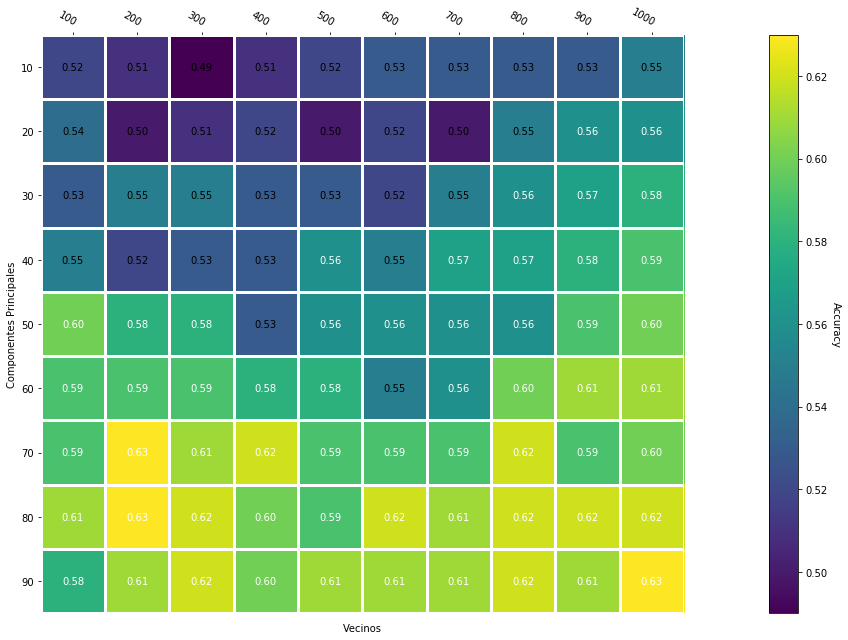
\includegraphics[width=\textwidth]{./img/parameters-search-small.png}
  \centering
  \caption{Resultado de la busqueda local sobre cada región
    \textbf{pequeña} de k100x$\alpha$10. Usando la implementación de
    sklearn. En cada una de las celdas, se corrió una búsqueda local,
    comenzando en el valor mostrado en los ejes hasta alcanzar un
    máximo local. El promedio de corridas es aproximadamente de 8,
    versus una cantidad de puntos de \textbf{1000}. Se muestran sobre
    el color, el accuracy logrado por el máximo local.}
  \label{fig:param-small}
\end{figure}

\begin{figure}[h]
  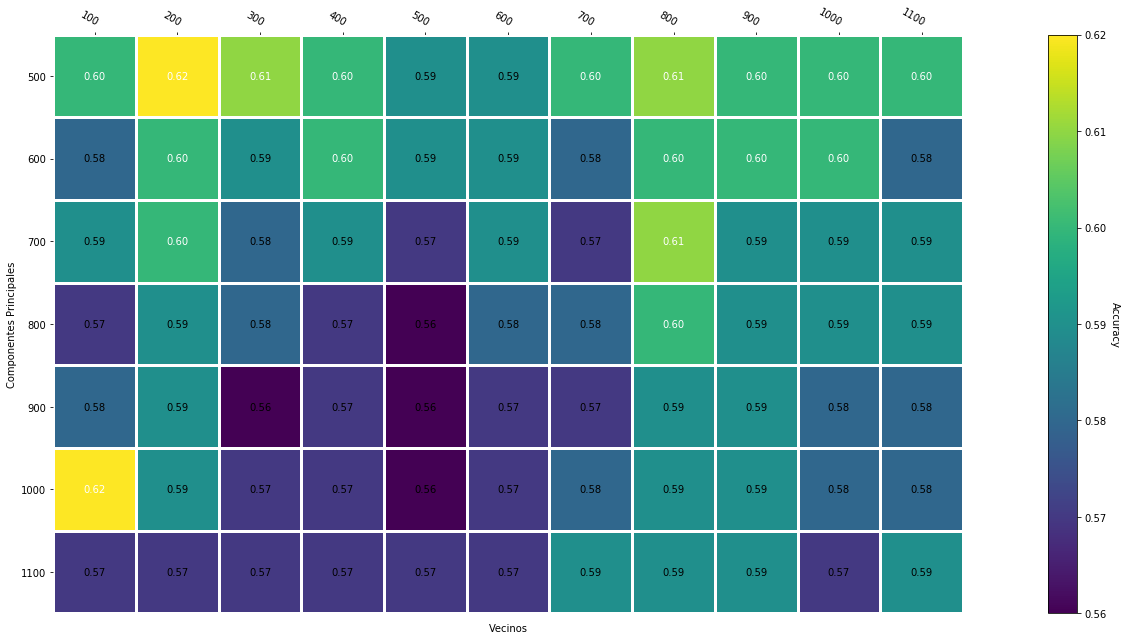
\includegraphics[width=\textwidth]{./img/parameters-search-big.png}
  \centering
  \caption{Resultado de la busqueda local sobre cada región
    \textbf{grande} de k100x$\alpha$100. Usando la
    implementación de sklearn. En cada una de las celdas, se corrió
    una búsqueda local, comenzando en el valor mostrado en los ejes
    hasta alcanzar un \textbf{máximo local}. El promedio de corridas
    es aproximadamente de 12, versus una cantidad de puntos de
    \textbf{10000}. Se muestran sobre el color, el accuracy logrado
    por el máximo local.}
    \label{fig:param-big}
\end{figure}
